\chapter{Résultats}
\chaptermark{Résultats}
\label{chapter:resultats}
	
	\section{Introduction}

		Nous avons désormais implémenté tous les éléments de notre simulateur, et nous allons donc pouvoir à présent tester le bon fonctionnement de notre système complet. Cela va nous permettre de tester que les différentes briques logicielles s'interfacent bien toutes ensemble et que le simulateur a un comportement physique correct.
		
		Dans un premier temps, nous allons vérifier que le système respecte les exigences présentées dans le Chapitre~\ref{chapitre:systeme}, ainsi que le comportement des robots et de l'environnement développés dans les Chapitres~\ref{chapitre:environnement} et \ref{chapitre:robots}.

		Ensuite, nous nous pencherons sur la comparaison du simulateur avec des expérimentations faites avec \argos{}, afin de déterminer si les résultats de simulations sont proches du comportement réel du robot, et si ce système permettrait bien de réduire les temps de développements en réduisant le nombre d'essais en conditions réelles à réaliser pour valider de nouvelles fonctionnalités.

	\section{Respect des exigences}

		\subsection{Introduction}

			Nous allons analyser et critiquer dans ce chapitre les résultats produits par notre simulateur. Nous allons nous intéresser principalement au robot \argos{}, d'abord parce que c'est sûr ce robot que ce sont principalement concentrés les efforts de développements pendant la durée de mon stage, mais aussi parce qu'outre les développements que j'ai pu réaliser pour ce robot (notamment au niveau du crochet de levage qui est un composant propre à \atoll{}), la conception de ce robot est en train d'être remaniée et la description \textit{URDF} de ce robot n'est pas encore aboutie. De ce fait, la simulation des composants est prête, car elle est aussi utilisée dans \argos{}, mais l'intégration de ces composants pour former le robot \atoll{} n'est pas encore réalisée.

		\subsubsection{Etat du simulateur}

			La fonction contrainte \textbf{FC1} prévoit de laisser la possibilité à l'utilisateur de connaître l'état des \gls{ROV}s et de l'environnement. A l'aide des librairies \textit{ignition} que nous utilisons pour faire communiquer les briques logicielles ensemble, nous pouvons voir transiter les messages et ainsi connaître l'état des robots.

			Le Listing~\ref{listing:ign_services} en annexes montre qu'un utilisateur peut connaître l'état de l'environnement de simulation en lançant des requêtes au \textit{plugin} d'environnement, où l'on peut obtenir l'accélération, la vitesse, la hauteur d'eau, sa densité ou encore la poussée d'Archimède en fonction de la position passée en paramètre.
			
			Le Listing~\ref{listing:ign_topics} en annexes présente les topics sur lesquels transitent les informations de la \textit{Rovins}, des différents propulseurs et de la nacelle pour caméra.

		\subsection{Visualisation des robots}

			\gls{ROS2} propose \textit{RViz2} qui est un outil qui permettant de visualiser les robots et les données fournies par les capteurs. Il est systématique de retrouver dans les packages de description de robots pour \gls{ROS2} un fichier de configuration permettant de visualiser le robot dans \textit{RViz2}. Pour notre simulateur, cela correspond à la fonction contrainte \textbf{FC3}. La Figure~\ref{fig:argos_rviz} présente \argos{} dans ce logiciel et montre qu'on est bien capable de visualiser le robot, l'état des actionneurs et des capteurs, car con peut voir les pâles des propulseurs tourner, l'orientation de la nacelle de la caméra ainsi que les images produites par les caméras.

			\begin{figure}[!htb]
				\centering
				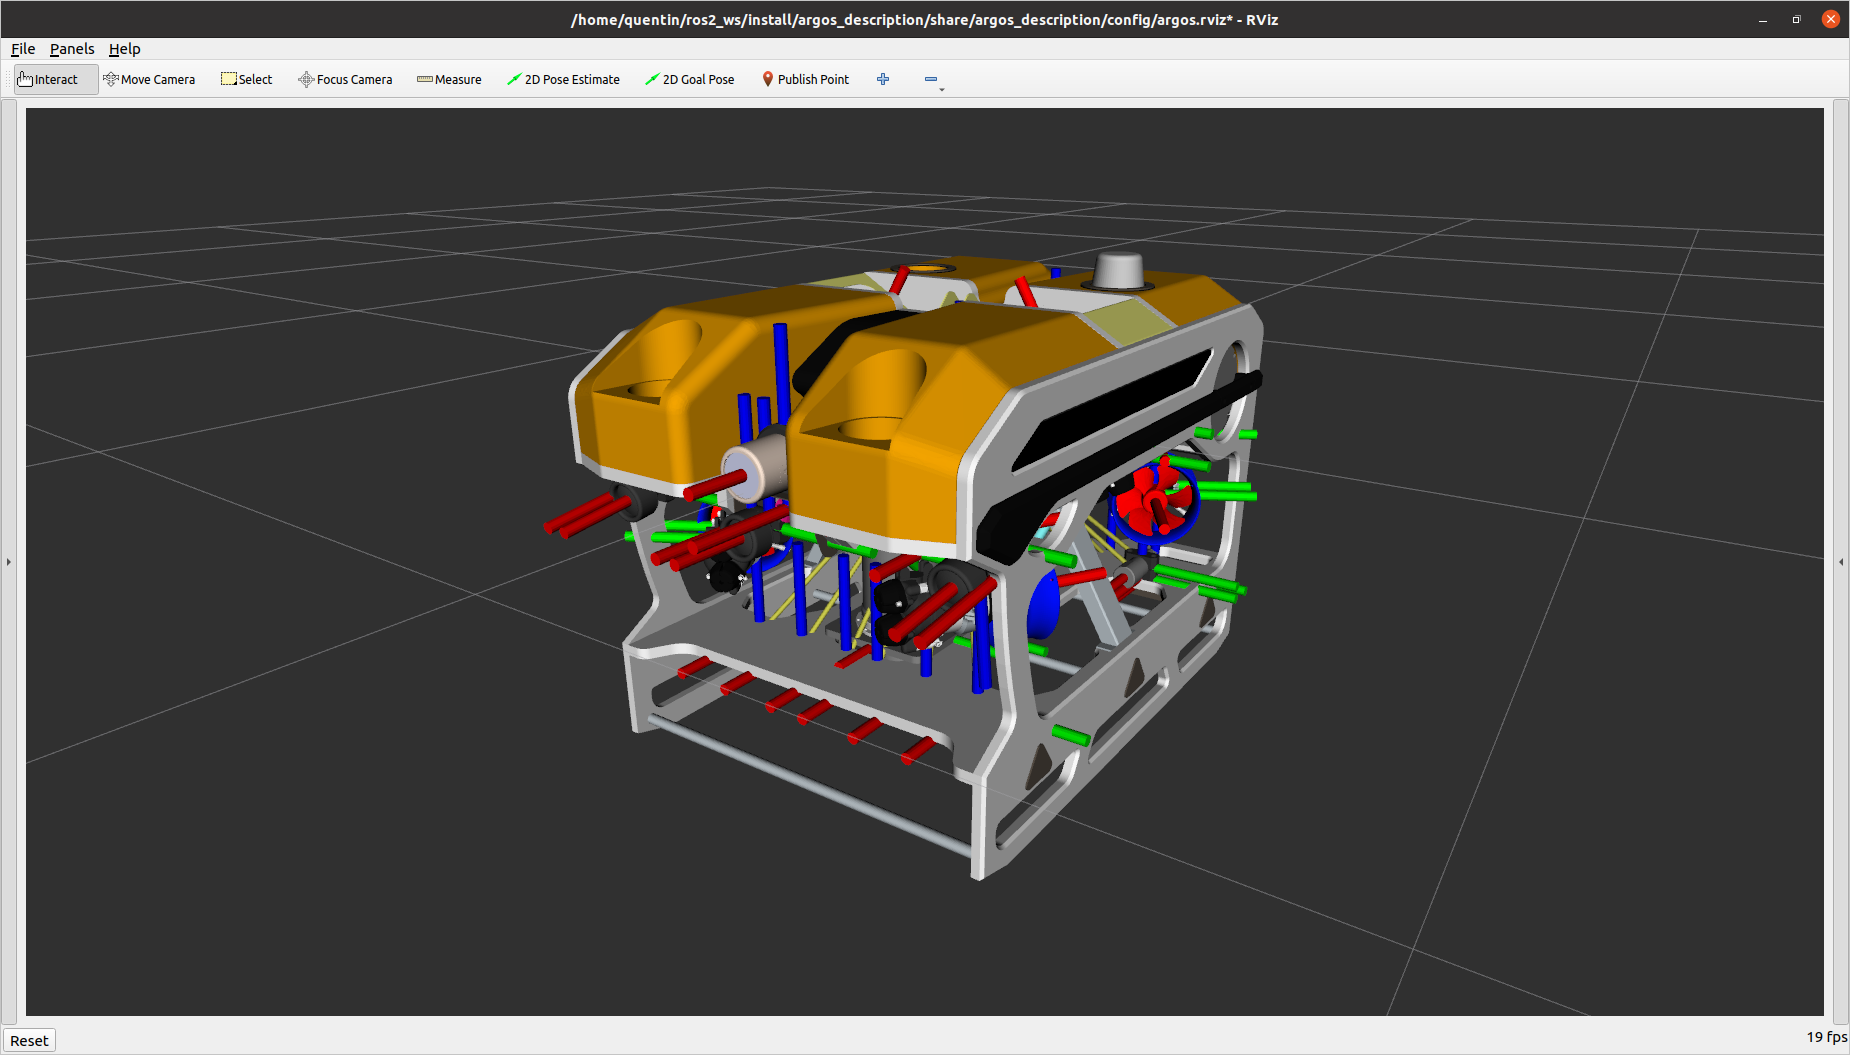
\includegraphics[width=0.6\textwidth]{imgs/argos_rviz.png}
				\caption{Visualisation d'\argos{} dans \textit{RViz2}}
				\label{fig:argos_rviz}
			\end{figure}

		\subsection{Invocation des robots dans l'environnement de simulation}

			Pour tester la cohérence du simulateur, nous allons tester l'invocation d'\argos{} dans l'environnement marin avec des vagues. La Figure~\ref{fig:argos_sea} présente ainsi ce robot dans l'eau, et on est en mesure de vérifier que la dynamique semble correcte et que toutes les briques logicielles sont bien interfacées. Cela permet de vérifier une partie des fonctions principales \textbf{FC1} et \textbf{FC2}. Les coefficients de trainée hydrodynamique et de masse ajoutée sont estimés à l'aide de données d'essais et pourront être améliorés par la suite en utilisant des logicielles de mécanique des fluides numérique.

			\begin{figure}
				\centering
				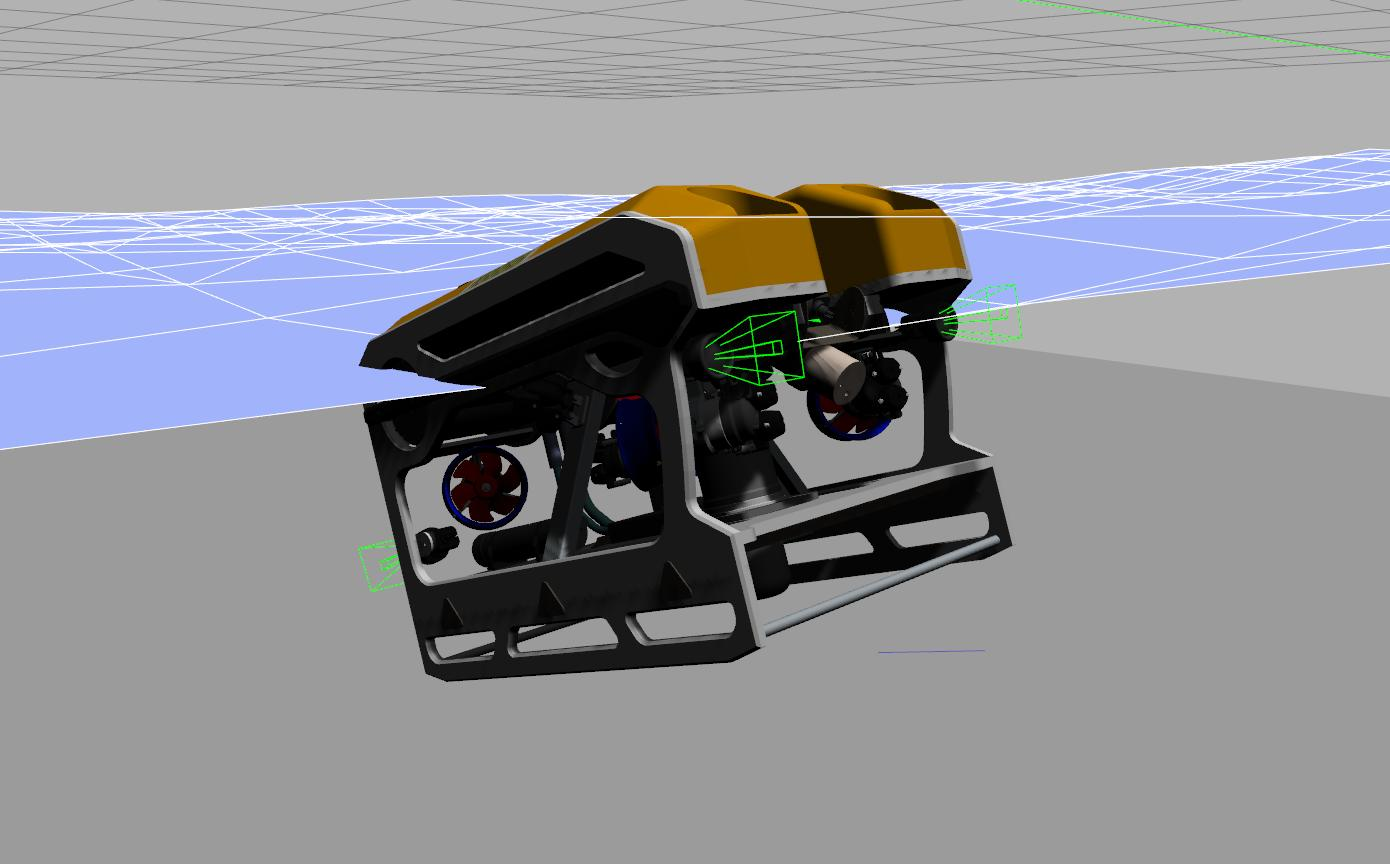
\includegraphics[width=0.6\textwidth]{imgs/argos_gazebo_sea.jpg}
				\caption{\argos{} dans son environnement marin simulé}
				\label{fig:argos_sea}
			\end{figure}

		\subsection{Rosace d'\argos{}}

			\argos{} a réalisé durant un essai des aller-retours avec une rotation de 3 degrés à chaque fois qu'il faisait demi-tour. Nous avons placé le robot à 10 mètres sous la surface afin de ne pas être impacté ni par les vagues ni par l'ombilical. Le mouvement dans le repère du monde ressemble globalement à des aller-retours entre deux points, mais si on trace la trajectoire dans le repère d'\argos{} on obtient une rosace. Les résultats de cet essai est visible sur la Figure~\ref{fig:rosace_argos} et il a permis de tester le mouvement du robot dans son plan transverse suivant une multitude d'angles de déplacement par pas de 3 degrés et sur un espace restreint dans le repère du monde.

			\begin{figure}[!htb]
				\centering
				\begin{subfigure}[t]{0.48\textwidth}
					\centering
					\includegraphics[width=\textwidth]{build/imgs/rosace_global.pdf}
					\caption{Dans le repère du monde}
				\end{subfigure}
				\hfill
				\begin{subfigure}[t]{0.48\textwidth}
					\centering
					\includegraphics[width=\textwidth]{build/imgs/rosace_local.pdf}
					\caption{Dans le repère d'\argos{}}
				\end{subfigure}
				\caption{Rosace réalisée par Argos}
				\label{fig:rosace_argos}
			\end{figure}

			L'idée a été de refaire le même essai avec le simulateur afin de tester la dynamique du robot. Pour ce faire, nous avons utilisé la même architecture de contrôle afin de tester la possibilité de s'interfacer avec l'implémentation logicielle. L'architecture logicielle de l'essai est présenté sur la Figure~\ref{fig:sa_rosace}. On voit un n\oe ud en charge de publier les \textit{Waypoints} que le robot devra suivre, qui va être comparé à l'état actuel du robot simulé dans le n\oe ud \textit{Feedback Linearization} basé sur un correcteur Proportionnel-Intégral-Dérivé afin de déterminer un \textit{Wrench}, qui est l'ensemble des forces et des couples qui vont devoir être appliqués au robot. Enfin, le n\oe ud \textit{Thrust Allocation} s'occupe d'allouer la puissance des propulseurs en fonction des efforts requis, et ainsi générer les commandes qui seront transmises aux propulseurs simulés.

			\begin{figure}[!htb]
				\centering
				\includegraphics[width=0.8\textwidth]{build/diagrams/sa_rosace.pdf}
				\caption{Architecture logicielle de l'essai dynamique}
				\label{fig:sa_rosace}
			\end{figure}

			Après avoir réalisé l'essai, on obtient les résultats visibles sur la Figure~\ref{fig:rosace_argos_simulation}. On remarque que l'essai dans le repère monde est beaucoup moins perturbé que l'essai réel. Cela est probablement dû au fait que lors de l'essai réel il y avait peut-être un faible courant qui est venu perturber le robot par exemple. On remarque aussi la présence de dépassements des \textit{waypoints} par le robot à chaque aller-retour, comparé au robot réel. Cela pourrait venir d'une sous-estimation des coefficients des forces hydrodynamiques, comme la masse ajoutée et la traînée. De ce fait, les réglages des coefficients du correcteur Proportionnel-Intégral-Dérivé utilisé pendant l'essai était peut-être trop important pour le simulateur qui avait moins de frottements. Enfin, comme nous l'avons remarqué, l'expression des efforts hydrodynamiques appliqués au robot ne sont vraies qu'en régime permanent et sont contestables en régime transitoire. Cette approximation des forces peut avoir un impact au démarrage et pendant les phases de ralentissement du robot à l'approche du \textit{waypoint}, ce qui pourrait expliquer les dépassements.

			\begin{figure}[!htb]
				\centering
				\begin{subfigure}[t]{0.48\textwidth}
					\centering
					\includegraphics[width=\textwidth]{build/imgs/rosace_global_simulation.pdf}
					\caption{Dans le repère du monde}
				\end{subfigure}
				\hfill
				\begin{subfigure}[t]{0.48\textwidth}
					\centering
					\includegraphics[width=\textwidth]{build/imgs/rosace_local_simulation.pdf}
					\caption{Dans le repère d'\argos{}}
				\end{subfigure}
				\caption{Rosace réalisée par Argos en simulation}
				\label{fig:rosace_argos_simulation}
			\end{figure}

	\section{Conclusion}

		En conclusion, nous avons montré dans ce chapitre que le système mis en place correspond aux exigences mises en place dans le Chapitre~\ref{chapitre:systeme}. Il reste cependant des ajustements à réaliser sur les coefficients qui permettent de régler la simulation pour ainsi mieux coller aux essais réels. De plus, il resterait à tester \atoll{} dans l'environnement de simulation afin de déplacer et de positionner des structures sous-marines simulées, ce qui n'a pas pu être fait pour l'instant, mais cette tâche va être poursuivie en suivant la démarche présentée pour \argos{} jusqu'à la fin de mon stage.